Eilera metodi \cite{burden2011} var izmantot neirona modeļa aproksimāciju aprēķināšanai pie jebkuras dotas vērtības. Piemērojot Eilera metodi \eqref{eq:izhi}, iegūst diskrēta laika vienādojumus membrānas potenciāla un atjaunošanās mainīgā vērtībām:
\begin{equation}
  \label{eq:discrete_uv}
  \begin{cases}
  v_{n + 1} = v_{n} + \Delta t(0{,}04v_{n}^{2} + 5v_{n} + 140 - u_{n} + I) \\
  u_{n + 1} = u_{n} + \Delta ta(bv_{n} - u_{n}).
  \end{cases}
\end{equation}

Eilera metode ir pirmās kārtas metode, kas nozīmē, ka lokālā diskretizācijas kļūda \(e(\Delta t)\) ir saistīta ar soļa lielumu kā \(e(\Delta t)=O(\Delta t^2)\), bet globālā diskretizācijas kļūda \(E(\Delta t)\) — kā \(E(\Delta t)=O(\Delta t)\). Jāņem vērā, ka lokālo kļūdu ietekme uzkrājas, jo turpmākajos aprēķinos tiek izmantotas noapaļotas vērtības. Praksē arī fiksētā komata noapaļošanas kļūda ietekmē globālo kļūdu, kura tad vairs nav lineāra attiecībā pret \(\Delta t\). Mazāka soļa izvēle sāks palielināt \(E(\Delta t)\), ja fiksētā komata precizitātes kļūda nebūs pietiekami maza salīdzinājumā ar soli. Šī ietekme jāņem vērā, nosakot atbilstošu fiksētā komata mainīgā un soļa lielumu.

Vienādojumu \eqref{eq:discrete_uv} var pārkārtot, aizstājot parametrus \(b\), \(I\) ar \(b^{*}=\Delta tb\) un \(I^{*}=\Delta tI\). Turklāt reizināšanu ar koeficientu \(0{,}04\Delta t\) var aizstāt ar nobīdes operāciju, izvēloties \(\Delta t\) tā, lai koeficients precīzi atbilstu divnieka pakāpei. Lai gan tas ierobežo laika soļa izšķirtspēju, reizināšanas operācijas ir precīzas un var izvēlēties arvien mazākas \(\Delta t\) vērtības. Abi realizējamie aprēķinu konveijeri kļūst par:
\begin{equation}
\label{eq:discrete_fe_uv}
\begin{cases}
  v_{n + 1} = v_{n} + v_{n}^{2}\gg n + 5\Delta tv_{n} + 140\Delta t - u_{n}^{*} + I^{*} \\
  u_{n + 1} = u_{n}^{*} + a(b^{*}v_{n} - u_{n}^{*}),
\end{cases}
\end{equation}
kur \(n\) ir pozīciju skaits, par kuru nobīdīt \(v^{2}_{n}\), un \(\gg\) ir binārā nobīde pa labi. Pārējās reizināšanas operācijas tiek saglabātas, un tās var realizēt ar aparatūras reizinātājiem vai \Gls{cordic} reizinātājiem, lai saglabātu precizitāti un parametru pielāgošanas elastību.

Vienādojuma (\ref{eq:discrete_fe_uv}) digitālās shēmas realizācija redzama \ref{fig:izhikevich_impl}. attēlā. Tā kā viens tipisks reizinātājs (piemēram, \Gls{dsp} kodols \textit{Xilinx Kintex} \Gls{fpga}) spēj veikt 18 bitu operācijas, katra reizinātāja operanda fiksētā komata vērtība ir ierobežota ar 18 bitu reprezentāciju. Šajā gadījumā viens reizinātājs tiek multipleksēts laikā, lai taupītu DSP bloku resursus. Salīdzinājumā ar citiem darbiem šis risinājums ļauj pielāgot laika soli uz lielāka aprēķinu latentuma rēķina. Var izmantot katru laika soli \(\Delta t = 2^{n}/0{,}04\), ja nobīdes operāciju skaits \(n\) ir vesels skaitlis.

\begin{figure}[htbp]
  \centering
  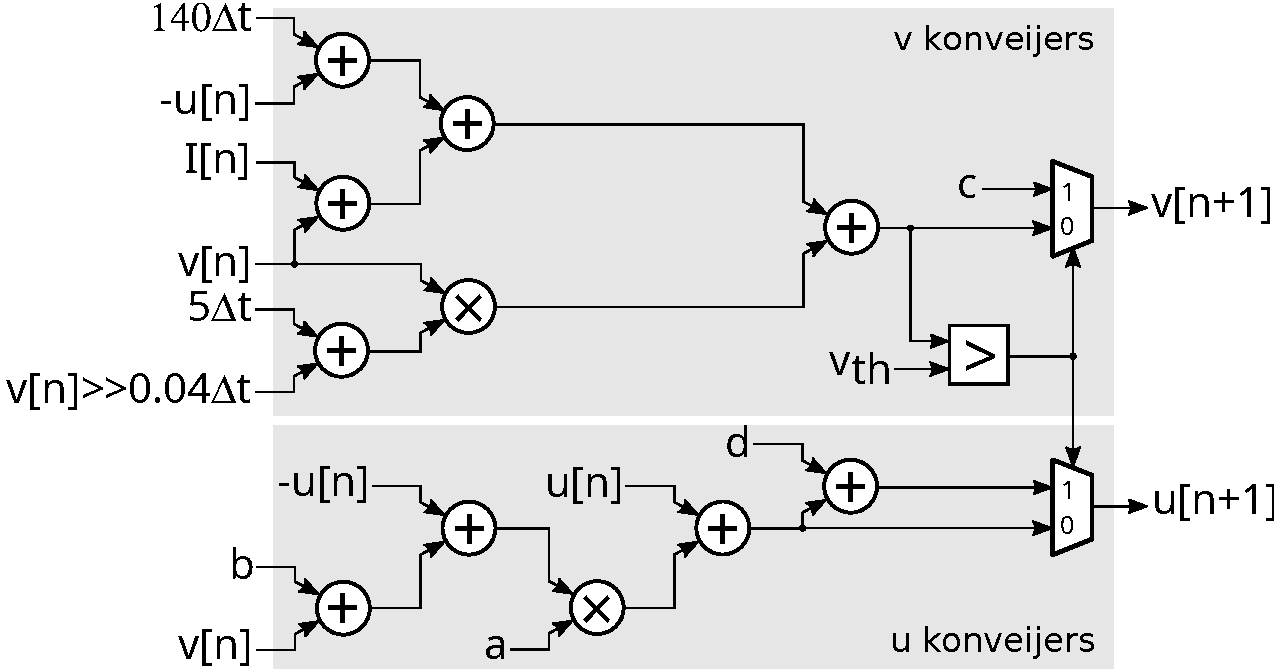
\includegraphics[width=0.7\columnwidth]{fig/lv/izh_impl_v2.pdf}
  \caption{Ižikeviča neirona realizācija, izmantojot tiešo Eilera metodi, kas optimizēta mainīgai precizitātei.}
  \label{fig:izhikevich_impl}

  \vspace{-0.5cm}
\end{figure}


